%!TEX root = ./report.tex

\section{Control and Observation}
Below you can find the implementation and results of the close-loop state feedback LQR controller.
Additionally, the results and implementation using a state observer are shown.
\subsection{LQR Design and Implementation}
Given the cost matrices and the linear system model, the LQR gain is computed using the MATLAB function \texttt{dlqr} or alternatively using the Ricatti recursive formula.
In order the observe the convergence of the Ricatti iteration, the singular values of the matrix $\bb{S}_n$ are observed.
For $\bb{Q}_1 = \diag (0, 1, 1, 1, 1)$ and $\bb{Q}_2 = \diag (1, 1)$ the convergence shows a profile as in Figure~\ref{fig:ricatti_svds}.
For other settings of the cost matrices the convergence looks slightly different.
Therefore, to have some when margin for guaranteed convergence upon cost function variance, the iteration number is set to $n_{iterations} = 2500$.

\begin{figure}[h]
	\centering
	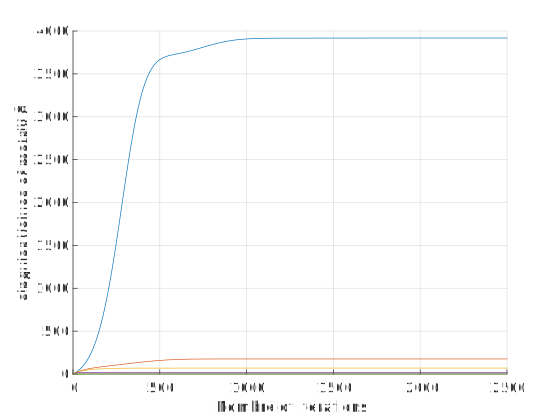
\includegraphics[width=.5\textwidth]{figures/svds.pdf}
	\caption{Evolution of the singular values of $\bb{S}_n$ during the Ricatti iteration.}
	\label{fig:ricatti_svds}
\end{figure}

When the LQR is computed the gain matrix is used as state feedback gain in a closed-loop fashion.
Figure~\ref{fig:lqr_closed} shows the implementation in Simulink.

\begin{figure}[h!]
	\centering
	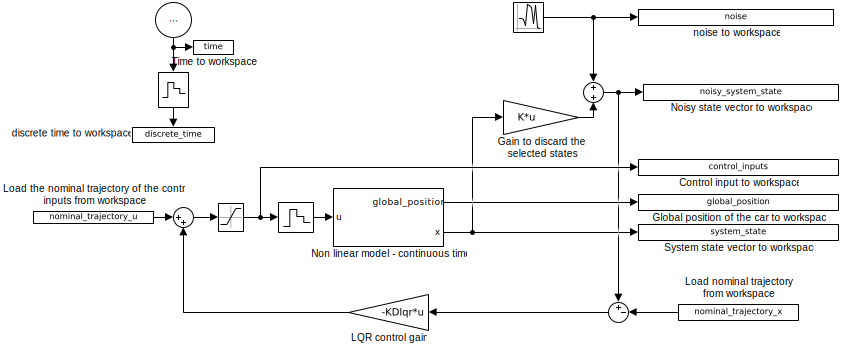
\includegraphics[width=\textwidth]{figures/lqr_closed_loop.pdf}
	\caption{Simulink implementation of the LQR state feedback controller. The LQR state feedback is added to the nominal trajectory for the control input and the sum signal is fed to the system model via a saturation and zero-order hold block. Then, the system output is distorted by noise and certain states are neglected. After subtracting the nominal state trajectory, the state signal is fed to the controller.}
	\label{fig:lqr_closed}
\end{figure}

\subsection{LQR Assessment with Ideal Information}

The closed-loop system including the controller is simulated using the second reference path and the results are presented in Figure~\ref{fig:lqr_closed_results}.
The simulation is run for different settings of the cost function, while the first weight for the state cost function is always zero.
On the top left (a) the identically weighted cost function is used and in (b) the weights for the angular values is increased by a factor of $10$.
The higher cost for angle errors leads to higher lateral deviations (state $2$) and lower control input for the steering angle at the same time.
In contrast to that, the lateral deviation is nearly ignored in (c) and only the heading error is considered for control.
In order to obtain a good performance the weight for the lateral deviation is increased and the behavior as in (d) is observed. 
At $t \approx 60s$ the vehicle slightly oscillates around the reference trajectory in the sharp curve, which is undesirable.
To get rid of the oscillation, the cost for steering is decreased, which results in an unstable behavior.
In particular, the system starts to oscillate uncontrollably at the critical sharp curve at $t \approx 60s$ (e).
Finally, by decreasing the weight for the lateral deviation again, a nice performance without oscillations for the settings shown in Figure~\ref{fig:lqr_closed_results} (f) is achieved.


\begin{figure}[h!]
	\centering
	\begin{subfigure}{0.32\textwidth}
		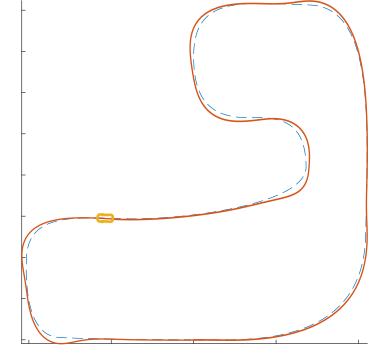
\includegraphics[width=.9\textwidth]{figures/clean_1_path.pdf}
		\includegraphics[width=\textwidth]{figures/clean_1_input.png}
		\subcaption{$\bb{Q}_1=\diag(0, 1, 1, 1, 1)$,\\$\bb{Q}_2=\diag(1, 1)$}
	\end{subfigure}
	\begin{subfigure}{0.32\textwidth}
		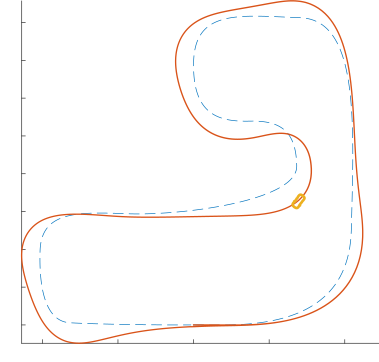
\includegraphics[width=.9\textwidth]{figures/clean_2_path.pdf}
		\includegraphics[width=\textwidth]{figures/clean_2_input.png}
		\subcaption{$\bb{Q}_1=\diag(0, 1, 100, 1, 100)$,\\$\bb{Q}_2=\diag(1, 100)$}
	\end{subfigure}
	\begin{subfigure}{0.32\textwidth}
		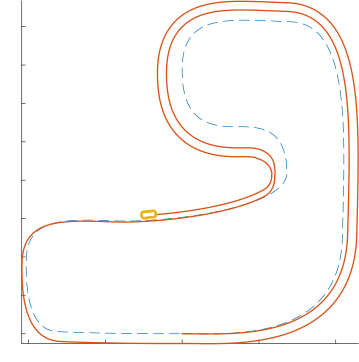
\includegraphics[width=0.9\textwidth]{figures/clean_6_path.pdf}
		\includegraphics[width=\textwidth]{figures/clean_6_input.png}
		\subcaption{$\bb{Q}_1=\diag(0, 10^{-4}, 500, 1, 1)$,\\$\bb{Q}_2=\diag(1, 0.5)$}
	\end{subfigure}
	\begin{subfigure}{0.32\textwidth}
		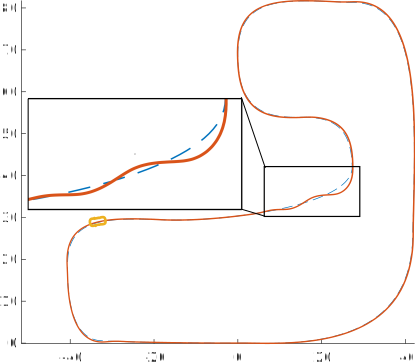
\includegraphics[width=0.9\textwidth]{figures/clean_3_path.pdf}
		\includegraphics[width=\textwidth]{figures/clean_3_input.png}
		\subcaption{$\bb{Q}_1=\diag(0, 100, 1, 1, 1)$,\\$\bb{Q}_2=\diag(1, 1)$}
	\end{subfigure}
	\begin{subfigure}{0.32\textwidth}
		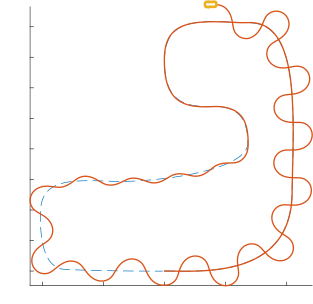
\includegraphics[width=0.9\textwidth]{figures/clean_5_path.pdf}
		\includegraphics[width=\textwidth]{figures/clean_5_input.png}
		\subcaption{$\bb{Q}_1=\diag(0, 100, 1, 1, 1)$,\\$\bb{Q}_2=\diag(1, 0.5)$}
	\end{subfigure}
	\begin{subfigure}{0.32\textwidth}
		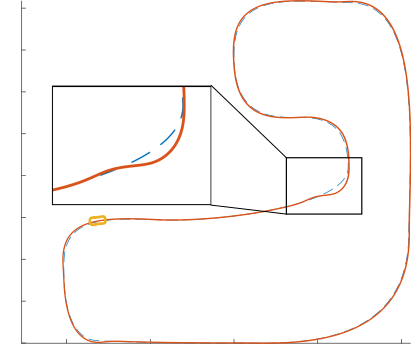
\includegraphics[width=0.9\textwidth]{figures/clean_4_path.pdf}
		\includegraphics[width=\textwidth]{figures/clean_4_input.png}
		\subcaption{$\bb{Q}_1=\diag(0, 20, 1, 1, 1)$,\\$\bb{Q}_2=\diag(1, 0.5)$}
	\end{subfigure}
	\caption{Resulting vehicle path (red line) as response to the reference trajectory (blue dashed line) using the closed-loop state feedback LQR controller. The experiment is run for different setting of the cost function.}
	\label{fig:lqr_closed_results}
\end{figure}

\subsection{LQR Assessment with Imperfect Information}

\paragraph{Adding Noise to the Fully Observable State} A white noise signal with standard deviations $\left[1, 1, 0.1745, 2, 0\right]$ is added to the state output as shown in Figure~\ref{fig:lqr_closed}.


\begin{figure}[h]
	\centering
	\begin{subfigure}{0.6\textwidth}
	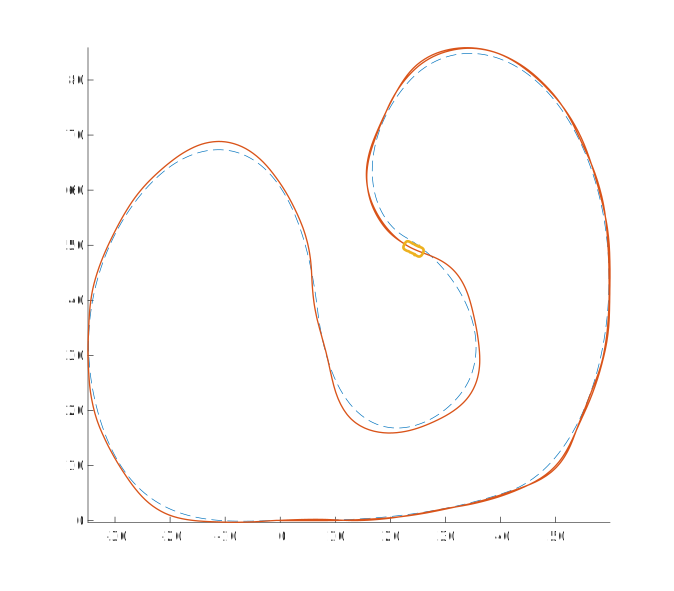
\includegraphics[width=\textwidth]{figures/noisy_1_path.pdf}
	\subcaption{Path}	
	\end{subfigure}
	\begin{subfigure}{0.49\textwidth}
	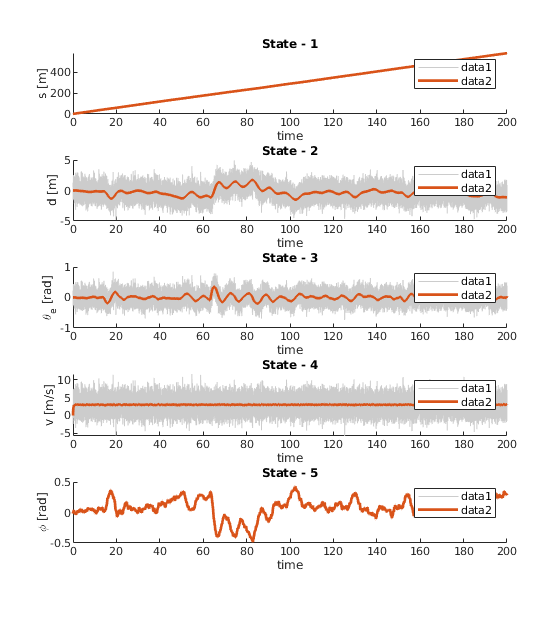
\includegraphics[width=\textwidth]{figures/noisy_1_states.pdf}
	\subcaption{States}	
	\end{subfigure}
	\begin{subfigure}{0.39\textwidth}
	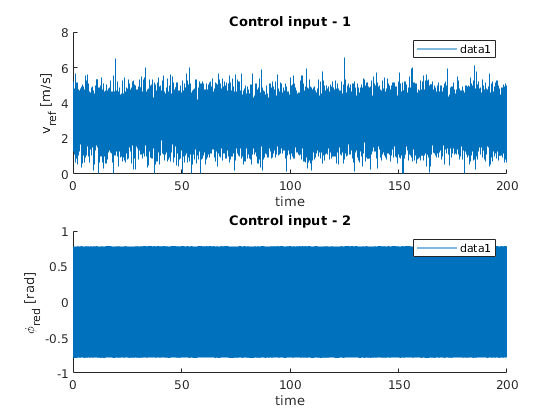
\includegraphics[width=\textwidth]{figures/noisy_1_inputs.pdf}
	\subcaption{Input}
	\end{subfigure}
	\caption{Performance of the LQR state feedback controller, when the state signal is distorted by noise.}
	\label{fig:noisy_states}
\end{figure}

\paragraph{Neglecting a State}

\begin{figure}[h]
	\centering
	\begin{subfigure}{0.49\textwidth}
	\includegraphics[width=\textwidth]{figures/partially_1_states.png}	
	\subcaption{States}
	\end{subfigure}
	\begin{subfigure}{0.49\textwidth}
	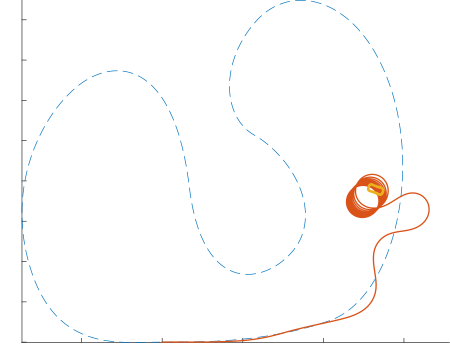
\includegraphics[width=\textwidth]{figures/partially_1_path.pdf}
	\subcaption{Path}	
	\end{subfigure}
	\caption{Performance of the LQR state feedback controller neglecting the heading error state for feedback.}
	\label{fig:partially_states}
\end{figure}

\subsection{State Observer}

\begin{figure}[h]
	\centering
	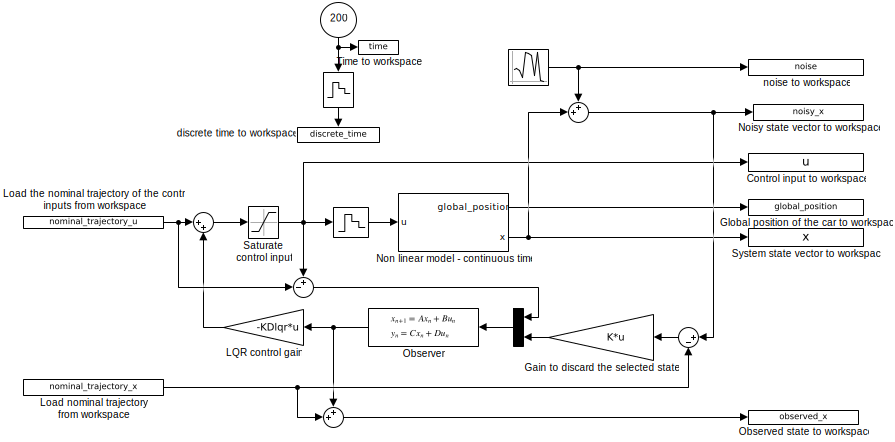
\includegraphics[width=\textwidth]{figures/lqr_observer.pdf}
	\caption{Simulink implementation of the LQR feedback controller combined with a state observer to infer neglected states.}
	\label{fig:lqr_and_observer}
\end{figure}
